\chapter{Robot Operating System - ROS}\label{cap:ros}

\begin{citacao}
``O Robot Operating System (ROS) é um conjunto de bibliotecas de software e ferramentas que te auxiliam na construção de aplicações em robótica. De drivers ao estado da arte de algoritmos, e com poderosas ferramentas de desenvolvimento, ROS tem o que você precisa para seu próximo projeto de robótica. E tudo é open source~\cite{Ros}''    
\end{citacao}

O ROS foi idealizado com o objetivo de ser um ambiente completo, de código aberto, para elaboração de sistemas robóticos. Largamente aceito e amplamente utilizado atualmente, os desenvolvedores se beneficiam da alta qualidade de código proporcionado pelo grande número de usuários e plataformas que aproveitam-se do ROS em seus projetos~\cite{RosIntro}. Uma ampla variedade de sensores e atuadores empregados na robótica também seguem essa tendência e oferecem suporte ao ROS através de seus drivers. O ROS fornece abstração de hardware, controle de baixo nível para dispositivos, funcionalidades e bibliotecas de uso comum, passagem de mensagens entre processos e gerenciamento de pacotes~\cite{rosEfetiveProgram}. Por esses motivos, o ROS é conhecido como um meta sistema operacional para robôs. Neste capítulo será apresentado o ROS e as vantagens do seu uso na concepção de novas plataformas robóticas.

A cada ano o ROS vem se consolidando como o framework padrão para o desenvolvimento de novos projetos de robótica, apesar de já possuir este status, o ROS possui uma história relativamente curta. O ROS teve início no Laboratório de Inteligência Artificial de Standord e em 2007 a companhia Willow Garage assumiu o seu desenvolvimento. A Willow Garage é uma empresa que desenvolve robôs pessoais e de serviços. Ela também é responsável pelo desenvolvimento de suporte a \textit{Point Cloud Library (PCL)}, que é uma biblioteca de software largamente usada para processamento de nuvens de pontos. Em Janeiro de 2010 a primeira versão do ROS foi lançada, desde então muitas outras versões foram lançadas. O ROS está sob as licenças BSD 3-Clause e Apache 2.0, que permite qualquer um modificar, reusar e distribuir códigos ROS~\cite{rosPYO}. Atualmente o ROS se encontra com uma versão estável do ROS2 e o ROS uma tem seu fim marcada para maio de 2015.



\section{Um sistema operacional para robôs}

De forma simplificada um sistema operacional tem como objetivo gerenciar os recursos do sistema computacional, ele atua como uma ponte entre esses recursos e o seu usuário, ou seja, o sistema operacional se faz necessário para disponibilizar às aplicações os recursos funcionais do sistema de forma padronizada, se tornando uma verdadeira camada de abstração entre os programas e o hardware. Windows, Ubuntu, para computadores pessoais e Android para smartphones, são exemplos de sistemas operacionais populares.

A comunidade da robótica em todo mundo tem feito grande progresso nos últimos anos. Hardware confiáveis e com menor custo têm sido ofertados em um nível nunca encontrado no passado, desde robôs móveis terrestres, passando por drones e até mesmo robôs humanóides estão disponíveis no mercado com relativa facilidade. O que pode ser até mais impressionante, a comunidade também tem desenvolvido algoritmos que permitem que estes robôs possuam um nível crescente de autonomia. Apesar desse rápido progresso, o desenvolvimento de robôs ainda representam um desafio para os desenvolvedores de softwares e grande parte desse desafio se deve a falta de padronização de um software específico para robótica, ou até mesmo um sistema operacional dedicado para robôs, como podemos encontrar em outros nichos, como os PCs e smartphones e o ROS tenta preencher essa lacuna.

O nome ROS vem da abreviação de Robot Operating System, mas seria o ROS um sistema operacional para robôs? Ele fornece abstração de hardware, controle de baixo nível para dispositivos, implementações de funcionalidades de uso comum, troca de mensagens entre processos, até um sistema de gerenciamento de pacotes. Além destas características o ROS está equipado com bibliotecas e ferramentas para escrever, compilar e rodar seus códigos~\cite{RosIntro}.

Apesar de todos os atributos que o caracterizam como um sistema operacional, o ROS não é um sistema operacional convencional, por ainda precisar rodar em um outro sistema operacional previamente instalado, o que faz com que o ROS seja conhecido como um meta-sistema operacional. Antes de ter o ROS em execução no robô é necessário instalar um sistema operacional, como por exemplo o Ubuntu. Com a distribuição Linux rodando é possível executar a instalação completa do ROS, sendo assim, todos os recursos fornecidos por um sistema operacional convencional podem ser utilizados pelo ROS, como sistema de gerenciamento de processos, sistema de arquivos, interface do usuário, compiladores entre outros. 

Para complementar esses recursos básicos do sistema operacional o ROS fornece funcionalidades específicas para o uso na robótica, tal como libraries para transmissão e recepção de dados para uma variedade de hardwares comumente utilizados em sistemas robóticos. Esse tipo de software é conhecido como middleware ou framework. Como pode ser visto na Figura~\ref{fig:rosmeta}, o ROS é o sistema auxiliar para controlar atuadores e sensores, com um nível de abstração de hardware dando suporte para o desenvolvimento de novas aplicações de robótica em sistemas operacionais convencionais.

\begin{figure}[ht]
	\caption{ROS um meta-sistema operacional}
	\begin{center}
		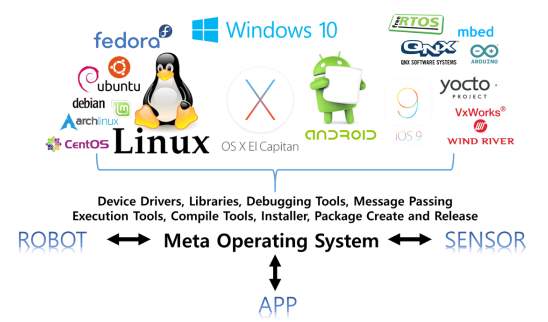
\includegraphics[scale=0.47]{imagens/metaOS.png}\\
		{\small \textbf{Fonte:} \citeonline{rosPYO}}
    \end{center}\label{fig:rosmeta}
\end{figure}



\section{Vantagens do ROS}


\subsection{Computacão distribuida}
\subsection{Reuso de Software}
\subsection{Testes Rápidos}

\section{Sistemas de aquivos}
ROS package
ROS Mensagens
ROS services

\section{Sistemas computacional ROS Graph level}
entendendo ROS node
ROS TOPIC
ROS master
ROS Parameters
Workspace ROS


\section{Community level- ROS ecosistema}


















No ROS um processo é conhecido como nó, que pode receber e enviar mensagens para se comunicar com outros nós através de uma rede rodando o protocolo TCPROS [3].










a busca por sistemas com um grau maior de autonomiaA robótica tem se caracterizádo pelo grande nível de percepção do ambiente e pelos sistemacomplexos de controle do movimentos 

Com essa distribuição de tarefas através de vários nós podemos criar sistemas cada vez mais complexos, apenas inserindo novos nós na rede, essa rede é gerenciada pelo ROS Master, que é apensas mais um nó do sistema, mas com a função de ser um servidor de nome e serviços para o restante dos nós. Ele identifica os nós na rede, assim todos os nós podem se comunicar com os outros através de conexões peer-to-peer, igura 1. Para desenvolver novas aplicações para o crescente grupo de pacotes ROS, o desenvolvedor deve respeitar os protocolos de comunicação da rede, as bibliotecas do ROS facilitam este trabalho, por já fornecer funções prontas para o desenvolvimento de novos códigos compatíveis e que possam se registrar na rede. Detalhes dos  rotocolos e interno podem ser visto em (ROS, 2011a), (ROS, 2018) e (ROS, 2011b).

% \chapter{Robot Operating System - ROS}\label{cap:ros}

Desenvolver um robô não é algo trivial, atividades que seriam facilmente executadas por nós, seres humnos, como por exemplo, andar de um ponto ao outro de uma sala, do ponto de vista de um robô pode ser um trabalho extremamente árduo. Montar o sistema que possibilite o robô executar as funções pra o qual foi projetado pode facilmente necessitar de um arranjo complexo entre componetes de software e hardware e que pode variar bastante dependendo do ambiente ao qual o robô será exposto. Sendo assim, o desenvolvimento de um sistema robôtico completo necessita de uma conhecimento abrangente e de áreas distintas.  

Nesse paronama que o ROS foi concebido, com o objetivo de  ser um um ambiente completo para desenvolvimento de sistemas robôticos, facilitando o desenvolvimento com o máximo de reuso de código possibilitando o mínimo de mudanças na adaptação um sistema a um novo ambiente ou até mesmo no desenvolvimento de uma nova plataforma. Atualmente o ROS é um framework bem aceito e amplamente utilizado não apenas na comunidade acadêmica mas também na industria. Desenvolvido originalmente em 2007 no \textit{Stanford Artificial Intelligence Laboratory - SAIL}, a partir de 2008 o ROS foi continuado pela Willow Garage, entretanto em 2012 com a criação da \textit{Open Source Robotics Foundation, Inc. - OSRF} os ROS e projetos parceiros como o Gazebo passaram a ser mantidos pela própria OSRF, que continua o desenvolvimento adicionando novas fancionalidades ao projeto. Além disso muitas instituições de pesquisa adaptaram seus projeto ao ROS, aumentando a cada ano o número de pesquisadores e desenvolvedores trabalhando no aperfeiçoamento do ROS. No site oficial do ROS podemos ver uma lista com diverssas plataformas que utilizam o ROS em seus projetos. http://wiki.ros.org/Robots

Muitos dos sensores e atuadores usados na robótica já são suportados pelo ros e o número de dispositivos compatíveis aumenta a cada ano. Algumas companias se beneficiam pelo fato de muitos deste dispositivos fazerem uso de hardware aberto e o software exitente também pode ser reutilizado a custo zero. Fazendo com que o processo de desenvolvimento de novos hardware periféricos usados na robótica também acelere.




Um sistema operacional para robôs

De forma simplificada um sistema operacional tem como objetivo gerenciar os recursos de um sistema computacional, ele atua como uma ponte entre esses recursos e o ultilizador, ou seja, o sistema operacional se faz necessário para disponibilizar às aplicações os recursos 
funcionais do sistema de forma padrinzada, se tornando uma verdadeira camada de abstração entre os programas e o hardware. Windows, Ubuntun, para computadores pessoais e Android para smartphones, são exemplos de sistemas operacionais populares.

O nome ROS vem da abrviação de Robot Operating System, mas seria o ROS um sistema operacional para robôs? Ele fornece abstração de hardware, controle de baixo nível para dispositivos, implementações de funcionalidades de uso comum, troca de mensagens entre processos, até um sistema de gerenciamento de pacotes. Além destas características o ROS está equipado com bibliotecas e ferramentas para escrever, compilar e rodar seus códigos. %http://www.ros.org/ROBOT PROGRAMMING \cite{rosPYO}%

Apesar de todos estes atributos, que caracterizam um sistema operacional, o ROS ainda precisa rodar sobre um outro sistema operacional previamente instalado, o que faz com que o ROS seja conhecido como um meta-sistema operacional. Antes de ter o ROS em execução no robô é necessário instalar um sistema operacional, como por exemplo o Ubuntu. Com a distribuição linux rodando é possível executar a instalação completa do ROS, sendo assim, todos os recursos fornecidos por um sistema operacional convencional podem ser utilizados pelo ROS, como sistema de genrenciamento de processos, sistema de arquivos, interface do usuário, compiladores entre outros. Para complementar esses recursos básicos do sistema operacional o ROS fornecer funcionalidades especificar para o uso na robótica, tal como libares para transmissão e recepção de dados para uma variedade de hardwares comumnete utilizados em sistemas robóticos. 

In addition to the basic features provided by Linux, ROS provides essential functions required for robot application programs as libraries such as data transmission/reception 
%among heterogeneous hardware, scheduling, and error handling.


This type of software is also called middleware or software framework. As a meta-operating system, ROS is developing, managing, and providing application packages for various purposes, and it has formed an ecosystem that distributes packages developed by users. 
As described in Figure 2-1, ROS is a supporting system for controlling a robot and sensor with a 
% hardware abstraction and developing robot application based on existing conventional operating systems.

% Tendo uma visão geral da função de um sistema operacional, podemos apontar porque o ROS é
% chamado de um meta-sistema operacional para robôs e não um sistema operacional verdadeiro
% como seu próprio nome indica, que é a abreviação de Robot Operating System. Apesar de fornecer 
% serviços que um sistema operacional precisa fornercer o ROS ainda precisa de um sistema 
% operacional padrão, como por exemplo o Ubuntu, para ser executado
Conceitos importantes

It uses graph architecture with a centralized topology, where processing takes place in nodes that may receive and send messages to communicate with other nodes on the graph net. A node is any process that can read data from a sensor, control an actuator, or run high level, complex robotic or vision algorithms for mapping or navigating autonomously in the
environment.\cite{rosEfetiveProgram}

One of the most frequently asked questions I received over the years in ROS-related seminars is to compare ROS with other robot software platforms (OpenRTM, OPRoS, Player, YARP, Orocos, CARMEN, Orca, MOOS, Microsoft Robotics Studio). A simple comparison with these platforms may be possible, but the comparison is not meaningful because they each have different purposes. As a user of ROS, I felt that the goal of ROS is to “build the development environment that allows robotic software development to collaborate on a global level!” That is to say, ROS is focused on maximizing code reuse in the robotics research and development, rather than orienting towards the so-called robot software platform, middleware, and framework. To support this, ROS has the following characteristics.


Distributed process: It is programmed in the form of the minimum units of executable processes (nodes), and each process runs independently and exchanges data systematically. Package management: Multiple processes having the same purpose are managed as a package so that it is easy to use and develop, as well as convenient to share, modify, and redistribute. Public repository: Each package is made public to the developer’s preferred public repository (e.g., GitHub) and specifies their license. API: When developing a program that uses ROS, ROS is designed to simply call an API and insert it easily into the code being used. In the source code introduced in each chapter, you will see that ROS programming is not much different from C++ and Python. These characteristics of ROS have allowed users to establish an environment where it is possible to collaborate on robotics software development on a global level. Reusing a code in robot 



